\documentclass[11pt]{amsart}
\usepackage{amsmath,amssymb,amsthm,mathtools,enumitem}
\usepackage[margin=1in]{geometry}
\usepackage{hyperref}
\usepackage{graphicx}

\newtheorem{theorem}{Theorem}[section]
\newtheorem{proposition}[theorem]{Proposition}
\newtheorem{corollary}[theorem]{Corollary}
\theoremstyle{remark}
\newtheorem*{remark}{Remark}

\title{The Cutting Plane: Every Line Through the Multiplication Table Is a Conic Section}
\author{Jeremy Ebert}
\address{Franklin County, Ohio, USA}
\date{2026}

\begin{document}
\maketitle

\begin{abstract}
Write out the ordinary multiplication table and draw a straight line through it. What curve does that line trace, once you plot the factor pairs it passes through in a natural coordinate system built from their sum, difference, and geometric mean? We answer this completely: the type of curve --- ellipse, parabola, or hyperbola --- is fixed by the sign of the line's coefficients, with the familiar circle traced by an anti-diagonal, and the familiar parabolas traced by a single row or column, appearing as two special cases of one proof rather than two separate facts. Along the way, the same coordinate system gives a one-line restatement of Fermat's 1643 factorization method and a short, visual re-derivation of the classical Dirichlet divisor summatory function.
\end{abstract}

\section{Introduction}

Write out the ordinary multiplication table: the grid whose entry in row $x$, column $y$ is $xy$, for $x,y=1,2,3,\dots$. Every entry sits at a lattice point $(x,y)$, and a natural question is what happens along a straight line drawn through this grid --- the diagonal $x=y$, an anti-diagonal $x+y=8$, a single row $x=3$, or any other line $ax+by=c$. Figure~\ref{fig:table_line} shows two examples, the anti-diagonal $x+y=8$ and a more general line $2x+5y=20$, three ways --- projected flat onto a plane of concentric circles, in the side-on $(X,T)$ projection introduced in Section~2, and, once the coordinate system of Section~2 turns the table into a cone, as an actual plane sliced through that cone in three dimensions, which is where the title of this note comes from --- with the whole table filled in out to the anti-diagonal $x+y=12$, so both examples sit comfortably inside a single frame. This note answers, completely, what curve each such line traces, and along the way uncovers an unexpected but elementary coordinate system for organizing several classical facts about factor pairs.

\begin{figure}[h]
\centering
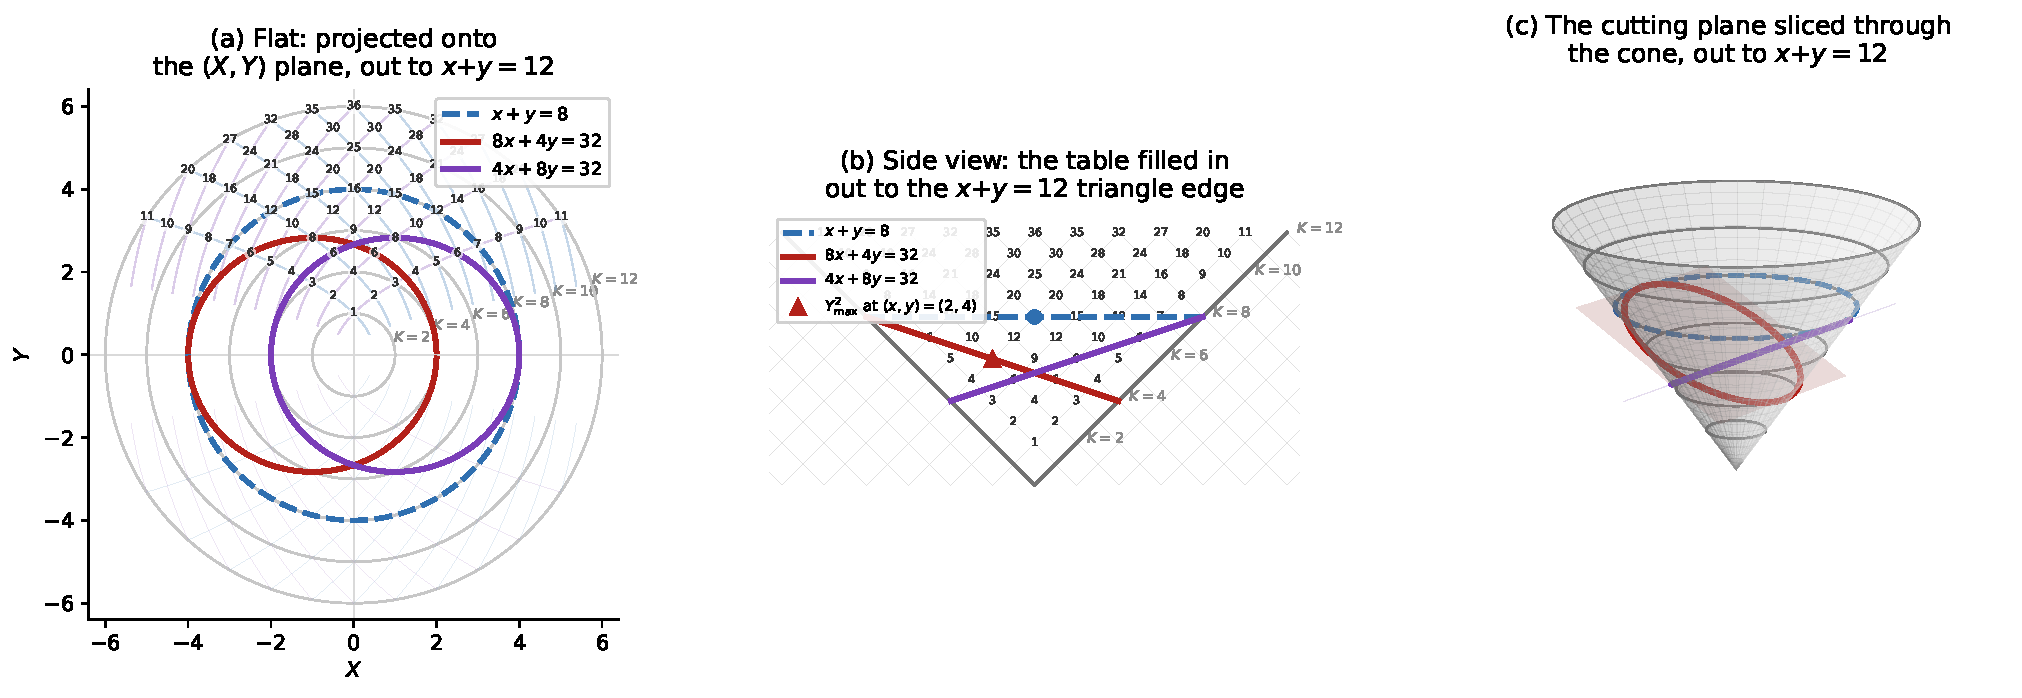
\includegraphics[width=\textwidth]{fig_cutting_plane_3panel.pdf}
\caption{Two lines through the multiplication table, shown three ways, with the whole table filled in out to the anti-diagonal $x+y=12$. (a) Projected onto the flat $(X,Y)$ plane: the concentric grey circles are the anti-diagonal circles $X^2+Y^2=T^2$ at fixed $T$, one for each even $K=x+y$ from $2$ to $12$; the faint blue and purple curves are the two mirror-image parabola families of Theorem~\ref{thm:conic}(b) --- rows (fixed $x$) and columns (fixed $y$) --- crossing to form a diamond mesh whose vertices are exactly the labeled table entries. The anti-diagonal $x+y=8$ (dashed blue) is exactly the $T=4$ circle, while the general line $2x+5y=20$ (solid red) projects down to an off-center oval, the shadow of the ellipse it traces on the cone --- entirely inside the outer $T=6$ circle. (b) The same two lines in the side-on $(X,T)$ projection of Section~2, with the same labeled lattice points filling the triangular mesh out to its edge at $x+y=12$: the anti-diagonal projects to the full horizontal segment $T=4$, $X\in[-4,4]$, since $T$ is fixed at $4$ while $X=(x-y)/2$ still ranges over every split of $8$ (the marked point $X=0$ is only the single AM-GM tangency case $x=y=4$ among the many points on that segment), while the general line becomes the straight cutting line $(a-b)X+(a+b)T=c$ seen edge-on. (c) The cutting plane $(a-b)X+(a+b)T=c$ sliced through the cone $X^2+Y^2=T^2$ in three dimensions, drawn out to the same $x+y=12$ boundary circle: the plane meets the cone in the ellipse of Theorem~\ref{thm:conic}, traced in red, alongside the anti-diagonal's circle (blue, dashed) for comparison.}
\label{fig:table_line}
\end{figure}

The coordinate system comes from an identity most readers have already seen, in a different guise. Given a pair of positive numbers $(x,y)$, their semi-difference $X=(x-y)/2$, geometric mean $Y=\sqrt{xy}$, and arithmetic mean $T=(x+y)/2$ always satisfy
\[
X^2+Y^2=T^2,
\]
which is nothing more than $\left(\frac{x-y}2\right)^2+xy=\left(\frac{x+y}2\right)^2$, verified by direct expansion. Geometrically, this is the right-triangle altitude theorem: if a right triangle's hypotenuse is split by the altitude from the right angle into segments of length $x$ and $y$, that altitude has length $\sqrt{xy}$ and the hypotenuse has length $x+y$. Setting $p=x,q=y$ recovers $Y$ as the altitude and $T=(x+y)/2$ as the semi-hypotenuse; $X$ is the signed distance from the midpoint of the hypotenuse to the foot of the altitude.

So every factor pair $(x,y)$, via $(X,Y,T)$, is secretly a point on the cone $X^2+Y^2=T^2$ in three-dimensional space --- and the question ``what does a line through the multiplication table look like?'' becomes ``what does a plane section of this cone look like?'' Fixing the anti-diagonal $x+y=K$ fixes $T=K/2$, and as $x$ ranges over $1,\dots,K-1$ the point $(X,Y)$ traces $K-1$ discrete points on the circle $X^2+Y^2=(K/2)^2$: the familiar picture of a multiplication table's anti-diagonal, now recognized as a circle. Section~2 makes this precise; Section~3 answers the general question for an arbitrary line; Sections~4 and~5 show what the same coordinate system buys classically, recovering Fermat's factorization method and the Dirichlet divisor summatory function as immediate consequences.

\section{Mean-Value Coordinates and the Conic Identity}

For a factor pair $(x,y)$ with $x,y>0$, define
\begin{equation}
X=\frac{x-y}2,\qquad Y=\sqrt{xy},\qquad T=\frac{x+y}2. \tag{2.1}
\end{equation}
These satisfy the AM--GM identity
\begin{equation}
X^2+Y^2=T^2. \tag{2.2}
\end{equation}
Fixing the anti-diagonal $x+y=K$ fixes $T=K/2$, so (2.2) restricts to the circle $X^2+Y^2=(K/2)^2$. As $x$ ranges over $1,\dots,K-1$ with $y=K-x$, the point $(X,Y)$ traces $K-1$ discrete points on that circle, with the diagonal point $x=y=K/2$ (when $K$ is even) sitting at the apex $X=0$, $Y=K/2$. Stacking these circles as $K$ varies produces the double-napped cone $X^2+Y^2=T^2$ in $(X,Y,T)$-space; this is the coordinate system used throughout.

\section{The General Conic Theorem}

The anti-diagonal $x+y=K$ is one line through the multiplication table among infinitely many. This section answers the natural question completely: what does an arbitrary line $ax+by=c$ produce?

\begin{theorem}\label{thm:conic}
Let $a,b$ be real numbers, not both zero, and $c$ a real number, and consider the line $ax+by=c$ intersecting the multiplication table. On the cone $X^2+Y^2=T^2$, this line traces:
\begin{itemize}
\item an ellipse if $ab>0$, with the circle of Section~2 as the symmetric special case $a=b$;
\item a parabola if $ab=0$ --- the rows ($b=0$) and columns ($a=0$) of the table;
\item a hyperbola if $ab<0$ --- a family distinct from the constant-product hyperbolas of Section~4.
\end{itemize}
\end{theorem}

\begin{proof}
For $b\ne0$, solve $ax+by=c$ for $y=(c-ax)/b$ and substitute into $Y^2=xy$:
\begin{equation}
Y^2=\frac cb x-\frac ab x^2, \tag{3.1}
\end{equation}
a quadratic function of $x$ with leading coefficient $-a/b$. When $ab>0$ this coefficient is negative, so $Y^2$ rises from $0$, reaches a maximum, and returns to $0$ as $x$ ranges over its real domain: a bounded, non-degenerate real conic is an ellipse. The case $a=b$ is the anti-diagonal $x+y=c/a$, whose ellipse degenerates by symmetry to the circle of Section~2. When $ab<0$ the coefficient is positive, so $Y^2$ grows without bound: an unbounded hyperbola. The case $b=0$ (or $a=0$) is a row or column, treated next.
\end{proof}

\begin{proposition}[Rows and columns are parabolas]
For a row $x=c$, $X+T=c$ and $Y^2=c(T-X)$; for a column $y=c$, $T-X=c$ and $Y^2=c(X+T)$. Both are parabolas.
\end{proposition}

\begin{proof}
Substituting $x=c$ into $X=(x-y)/2$, $T=(x+y)/2$ gives $X+T=c$ identically, independent of $y$; writing $W=T-X$, we get $W=y$, so $Y^2=xy=cW$. This is the classical construction of a parabola as a conic section: the plane $X+T=c$ has normal vector $(1,0,1)$, and the cone has a generator direction $(-1,0,1)$ lying on it, since $(-1)^2+0^2=1^2$. Since $(1,0,1)\cdot(-1,0,1)=0$, the plane $X+T=c$ is parallel to that generator --- and slicing a cone with a plane parallel to (but not through) one of its own generators is exactly the classical definition of a parabola. Columns use the mirror generator $(1,0,1)$, by the same argument with $T-X=c$.
\end{proof}

Concretely: the row $x=1$ ($y=1,2,3,4,\dots$) satisfies $X+T=1$ throughout, with $Y^2=y$ taking the values $1,2,3,4,\dots$; the row $x=2$ satisfies $X+T=2$, with $Y^2=2y$ taking the values $2,4,6,8,\dots$; and so on for every row.

\begin{proposition}[Semi-axes and eccentricity, ellipse case]
For $ab>0$, $Y^2$ is maximized exactly at $x=c/(2a)$, where it equals $c^2/(4ab)$ --- and this maximum sits at the midpoint of the line's two axis intercepts, $(c/a,0)$ and $(0,c/b)$.
\end{proposition}

\begin{proof}
Differentiating (3.1) and setting the result to zero gives $x=c/(2a)$; substituting back gives $Y^2_{\max}=c^2/(4ab)$. The intercepts are $x=c/a$ (at $y=0$) and $x=0$ (at $y=c/b$), whose midpoint in $x$ is $c/(2a)$.
\end{proof}

For the line $2x+5y=20$ of Figure~\ref{fig:table_line} ($a=2,b=5,c=20$), this predicts the maximum at $(x,y)=(5,2)$, with $Y^2_{\max}=400/40=10$, matching $xy=5\cdot2=10$ exactly and matching the marked point in Figure~\ref{fig:table_line}(b).

The case $ab<0$ --- a line like $x-y=d$, a fixed difference rather than a fixed sum --- produces a hyperbola by the same mechanism run in reverse: the coefficient $-a/b$ in (3.1) is positive, so $Y^2$ grows without bound. This is a genuinely different construction from the constant-product hyperbolas of Section~4, arising from a linear rather than a multiplicative condition; we do not develop it further here beyond noting that Theorem~\ref{thm:conic} places the ellipse, the parabola, and this second hyperbola family under one proof.

\begin{remark}
Theorem~\ref{thm:conic} is itself a special case of the classical fact that any plane section of a quadric surface is a conic section; what it contributes is the explicit classification, by the sign of $ab$, for the specific family of planes that lines through the multiplication table happen to produce.
\end{remark}

\section{Constant-Product Curves and Fermat's Factorization Method}

A different, non-linear curve family fixes the product rather than a linear combination: $xy=N$. Since $Y^2=xy$, this fixes $Y^2=N$ in (2.2), giving
\begin{equation}
T^2-X^2=N. \tag{4.1}
\end{equation}
This is exactly Fermat's factorization method (1643): to factor an odd $N$, test successive integers $a\ge\lceil\sqrt N\rceil$ until $a^2-N$ is a perfect square $b^2$, at which point $N=a^2-b^2=(a-b)(a+b)$ is a factorization. The search terminates fastest when $N$ has a factor pair close to $\sqrt N$, i.e.\ when the corresponding $X$ is small. In the coordinates of Section~2, $a=T$ and $b=X$ exactly, so the constant-product curve $xy=N$ is the graph of every factorization Fermat's method could find, and (4.1) is simply that method's defining equation, restated three and a half centuries later in mean-value coordinates.

\section{The Divisor Summatory Function via Nested Gnomons}

The coordinate system of Sections~2--4 also gives a short, visual re-derivation of a classical object: the divisor summatory function $D(n)=\sum_{k=1}^nd(k)$, the number of lattice points $(x,y)$ with $x,y\ge1$ and $xy\le n$. Dirichlet's 1849 hyperbola method sums full rows or columns and removes the double-counted square of side $\lfloor\sqrt n\rfloor$. Here we anchor the same count on the diagonal $x=y$ instead --- the spine from which the circles of Section~2 radiate.

For each vertex $(u,u)$ with $1\le u\le\lfloor\sqrt n\rfloor$, form the L-shaped gnomon consisting of the vertex itself, a horizontal arm along $y=u$ out to the hyperbola at $x=\lfloor n/u\rfloor$ (containing $\lfloor n/u\rfloor-u$ points), and, by the symmetry of the region under $x\leftrightarrow y$, an identical vertical arm. The total count is
\begin{equation}
D(n)=\sum_{u=1}^{\lfloor\sqrt n\rfloor}\left[2\left\lfloor\frac{n-u^2}u\right\rfloor+1\right]. \tag{5.1}
\end{equation}
Expanding algebraically --- using $u^2/u=u$ to pull $u$ out of the floor function, then applying $\sum u=k(k+1)/2$ with $k=\lfloor\sqrt n\rfloor$ --- collapses this to
\begin{equation}
D(n)=2\sum_{u=1}^{\lfloor\sqrt n\rfloor}\left\lfloor\frac nu\right\rfloor-\lfloor\sqrt n\rfloor^2, \tag{5.2}
\end{equation}
exactly the textbook symmetric form of the Dirichlet hyperbola identity. So the gnomonic decomposition is algebraically equivalent to the classical derivation --- a re-indexing, not a new identity --- but it organizes the same sum around the axis of symmetry $x=y$, the same spine that anchors the circles of Section~2 and the ellipses and parabolas of Section~3.

\section{Discussion}

Sections~2--5 rest on one piece of elementary algebra, the AM--GM identity $X^2+Y^2=T^2$, and one classification theorem built on top of it: every line through the multiplication table produces a conic on the resulting cone, its type fixed by the sign of $ab$ (Theorem~\ref{thm:conic}). Circles and the row/column parabolas are now special cases of a single proof rather than two separate facts, and a genuine ellipse family comes along for free. Section~4 identifies the constant-product hyperbolas with Fermat's 1643 factorization method, and Section~5 shows the same coordinate system reorganizing the classical divisor summatory function around its own diagonal spine. The throughline is a single mechanism, stated once and used three times: every curve considered here is what results from intersecting a plane or a hyperbola with the quadric surface that $Y=\sqrt{xy}$ generates by definition.

\begin{thebibliography}{9}
\bibitem{Dickson} L.~E.~Dickson, \emph{History of the Theory of Numbers, Vol.~I}, Carnegie Institution, 1919, Ch.~14.
\bibitem{Dirichlet} P.~G.~L.~Dirichlet, \"Uber die Bestimmung der mittleren Werthe in der Zahlentheorie, \emph{Abh.\ K\"onigl.\ Preuss.\ Akad.\ Wiss.} (1849), 69--83.
\end{thebibliography}

\end{document}
